% ============================================================
% SECTION 1 - GIỚI THIỆU
% Bối cảnh → Phát biểu bài toán → Phân loại → Thị trường
% → Đối thủ → SWOT → Personas → USP & Winning Zone
% ============================================================
\section{Giới thiệu}

% ------------------------------------------------------------
% Slide giới thiệu app: logo + tên + mô tả tổng quan
% ------------------------------------------------------------
\begin{frame}
\vfill
\begin{center}
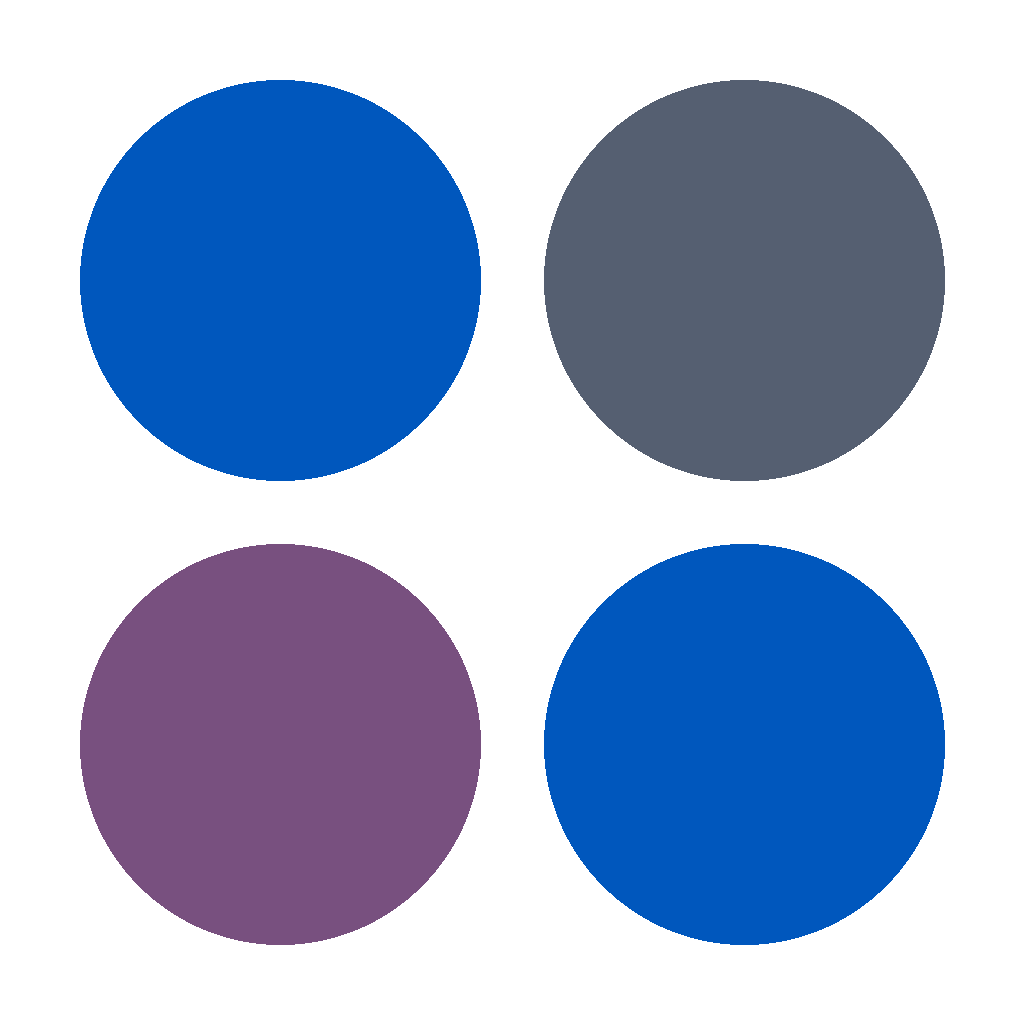
\includegraphics[height=2.9cm]{figures/onespace-logo-transparent.png}\\[2.5mm]
{\LARGE\bfseries\color{BKTemplate} OneSpace}\\[1.5mm]
{\small\bfseries\color{BKDark} Ứng dụng giải trí tích hợp 4-trong-1 trên Android}\\[4mm]
\begin{minipage}{0.86\textwidth}
\begin{exampleblock}{Mô tả tổng quan}
{\small Một ứng dụng duy nhất cho bốn nhu cầu giải trí: xem video, nghe nhạc, đọc tin và chơi minigame. Nội dung đi theo người dùng khi đổi hoạt động~--~nhạc chạy nền, video nổi, bài đọc thu thành thẻ~--~nên trải nghiệm liền mạch thay vì bốn ứng dụng rời rạc.}
\end{exampleblock}
\end{minipage}
\end{center}
\vfill
\end{frame}

% ------------------------------------------------------------
\subsection{Bối cảnh}
% ------------------------------------------------------------
\begin{frame}{Bối cảnh}
\begin{columns}[T]
\begin{column}{0.52\textwidth}
\footnotesize
\begin{itemize}\setlength{\itemsep}{3pt}
\item Điện thoại là thiết bị giải trí chính của người Việt:
      \textbf{137 triệu} kết nối di động (134\% dân số);
      \textbf{85,6 triệu} người dùng Internet (84,2\%)
\item 82\% người được khảo sát dùng TikTok trong 7 ngày gần nhất;
      dành \textbf{7,1 giờ/ngày} cho ứng dụng di động và dùng hơn \textbf{27 ứng dụng/tuần}
\item Mỗi loại nội dung một bộ ứng dụng riêng:
      Video (YouTube, TikTok\ldots), Âm nhạc (Spotify, Zing\ldots),
      Tin tức (VnExpress, Báo Mới\ldots), Minigame: rời rạc trên Facebook, YouTube Playables, Shopee\ldots
\end{itemize}
\end{column}
\begin{column}{0.44\textwidth}
\centering
\vspace{1mm}

\includegraphics[height=1.9cm,keepaspectratio=true]{figures/Bối cảnh-01.png}\\[3pt]

\includegraphics[height=1.9cm,keepaspectratio=true]{figures/Bối cảnh-02.png}\\[3pt]
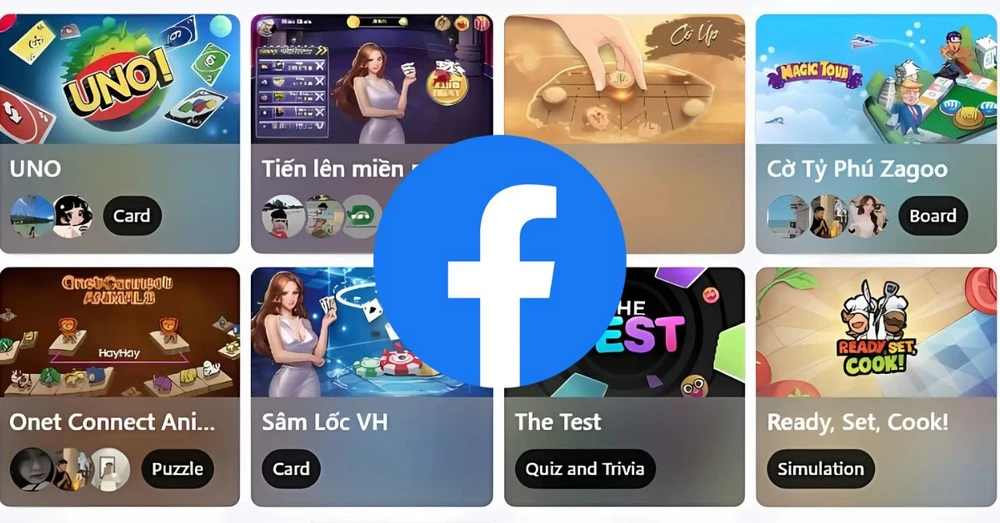
\includegraphics[height=1.9cm,keepaspectratio=true]{figures/Bối cảnh-03.png}
\end{column}
\end{columns}
\end{frame}

% ------------------------------------------------------------
\subsection{Phát biểu bài toán}
% ------------------------------------------------------------
\begin{frame}{Phát biểu bài toán}
\begin{columns}[T]
\begin{column}{0.54\textwidth}
\footnotesize
\begin{block}{Trải nghiệm đứt gãy (Context Switching)}
\begin{itemize}\setlength{\itemsep}{1pt}
\item Nội dung không theo người dùng khi đổi ngữ cảnh
\item Chế độ thu nhỏ picture-in-picture (PIP) tuỳ app
\item Khó phối hợp âm thanh
\end{itemize}
\end{block}
\vspace{-0.06cm}
\begin{block}{Tài khoản \& thông báo}
Đăng nhập nhiều lần, thông báo đẩy chồng chéo
\end{block}
\vspace{-0.06cm}
\begin{block}{Tài nguyên}
Nhiều ứng dụng chiếm nhiều không gian lưu trữ, RAM khi chạy nền, cạn pin
\end{block}
\end{column}
\begin{column}{0.43\textwidth}
\begin{alertblock}{Bài toán}
\small\itshape
``Làm thế nào để thiết kế một ứng dụng Android hợp nhất bốn phân hệ Streaming Video, Listening to Music, Reading News và Playing Minigames trong một trải nghiệm liền mạch, và giá trị khác biệt nào khiến người dùng chọn ứng dụng này thay vì tiếp tục dùng các ứng dụng quen thuộc hiện tại?''
\end{alertblock}
\end{column}
\end{columns}
\end{frame}

% ------------------------------------------------------------
\subsection{Phân tích bài toán và thu thập yêu cầu}
% ------------------------------------------------------------
\begin{frame}{Phân tích bài toán \& thu thập yêu cầu}
\begin{columns}[T]
\begin{column}{0.31\textwidth}
\begin{block}{\scriptsize\bfseries Nghiên cứu thị trường}
{\tiny
\begin{itemize}\setlength{\itemsep}{1.5pt}
\item DataReportal Digital 2026: 85,6~triệu người dùng Internet (84,2\%)
\item StatCounter 9/2026: Android 59,77\% thị phần di động
\item Q\&Me 2026: 7,1~giờ/ngày, 27+ app/tuần (mẫu 100 người dùng iPhone)
\end{itemize}}
\end{block}
\end{column}
\begin{column}{0.31\textwidth}
\begin{block}{\scriptsize\bfseries Phân tích app đối thủ}
{\tiny
\begin{itemize}\setlength{\itemsep}{1.5pt}
\item Dùng trực tiếp YouTube, TikTok, Mocha; đối chiếu 6 nền tảng gián tiếp
\item Ma trận tính năng 6 đối thủ $\times$ 4 dạng nội dung
\item 3.750 review App Store VN (2021--2026): pain point liền mạch lặp lại
\end{itemize}}
\end{block}
\end{column}
\begin{column}{0.31\textwidth}
\begin{block}{\scriptsize\bfseries Phân tích người dùng}
{\tiny
\begin{itemize}\setlength{\itemsep}{1.5pt}
\item 6 chân dung người dùng theo hành vi tiêu thụ nội dung
\item Pain: đứt gãy ngữ cảnh, khó phối hợp âm thanh, khó tiếp cận
\end{itemize}}
\end{block}
\end{column}
\end{columns}
\vspace{1mm}
\begin{block}{\scriptsize\bfseries Bằng chứng người dùng thật --- trích review App Store Việt Nam}
{\tiny
\begin{itemize}\setlength{\itemsep}{1pt}
\item \textbf{YouTube} (1/5$\bigstar$, 11/2026): ``\ldots không thu nhỏ video để vừa xem vừa dùng app khác, phải pause play lại mới được''
\item \textbf{Zing MP3} (2/5$\bigstar$, 10/2026): ``hay dùng để nghe nhạc khi chơi ff \ldots\ cứ ra sảnh lại mất nhạc''\quad·\quad \textbf{Zalo} (1/5$\bigstar$, 2026): ``spam liên tục \ldots\ mất tập trung''
\item \textbf{VnExpress} (1/5$\bigstar$, 2024): ``nặng tốn dung lượng, tốn pin dễ nóng máy''
\end{itemize}}
\end{block}
\vspace{0.8mm}
{\tiny\color{TextGray} Stakeholder: người dùng cuối (6 persona) $\cdot$ nhóm phát triển $\cdot$ nhà trường / GVHD $\cdot$ nền tảng (Google Play, AdMob). \quad Đầu ra: 76 tính năng $\rightarrow$ C1--C12 $\rightarrow$ 45 user story.}
\end{frame}

% ------------------------------------------------------------
\subsection{Phân loại ứng dụng}
% ------------------------------------------------------------
\begin{frame}{Phân loại ứng dụng}
\begin{columns}[T]
\begin{column}{0.52\textwidth}
\footnotesize
\begin{block}{Primary}
\textbf{Entertainment}
\end{block}
\vspace{1pt}
\begin{block}{Secondary}
\begin{itemize}\setlength{\itemsep}{1pt}
\item Music \& Audio
\item News \& Magazines
\item Video Players \& Editors
\item Games --- Casual / Puzzle / Trivia
\end{itemize}
\end{block}
\end{column}
\begin{column}{0.44\textwidth}
\centering
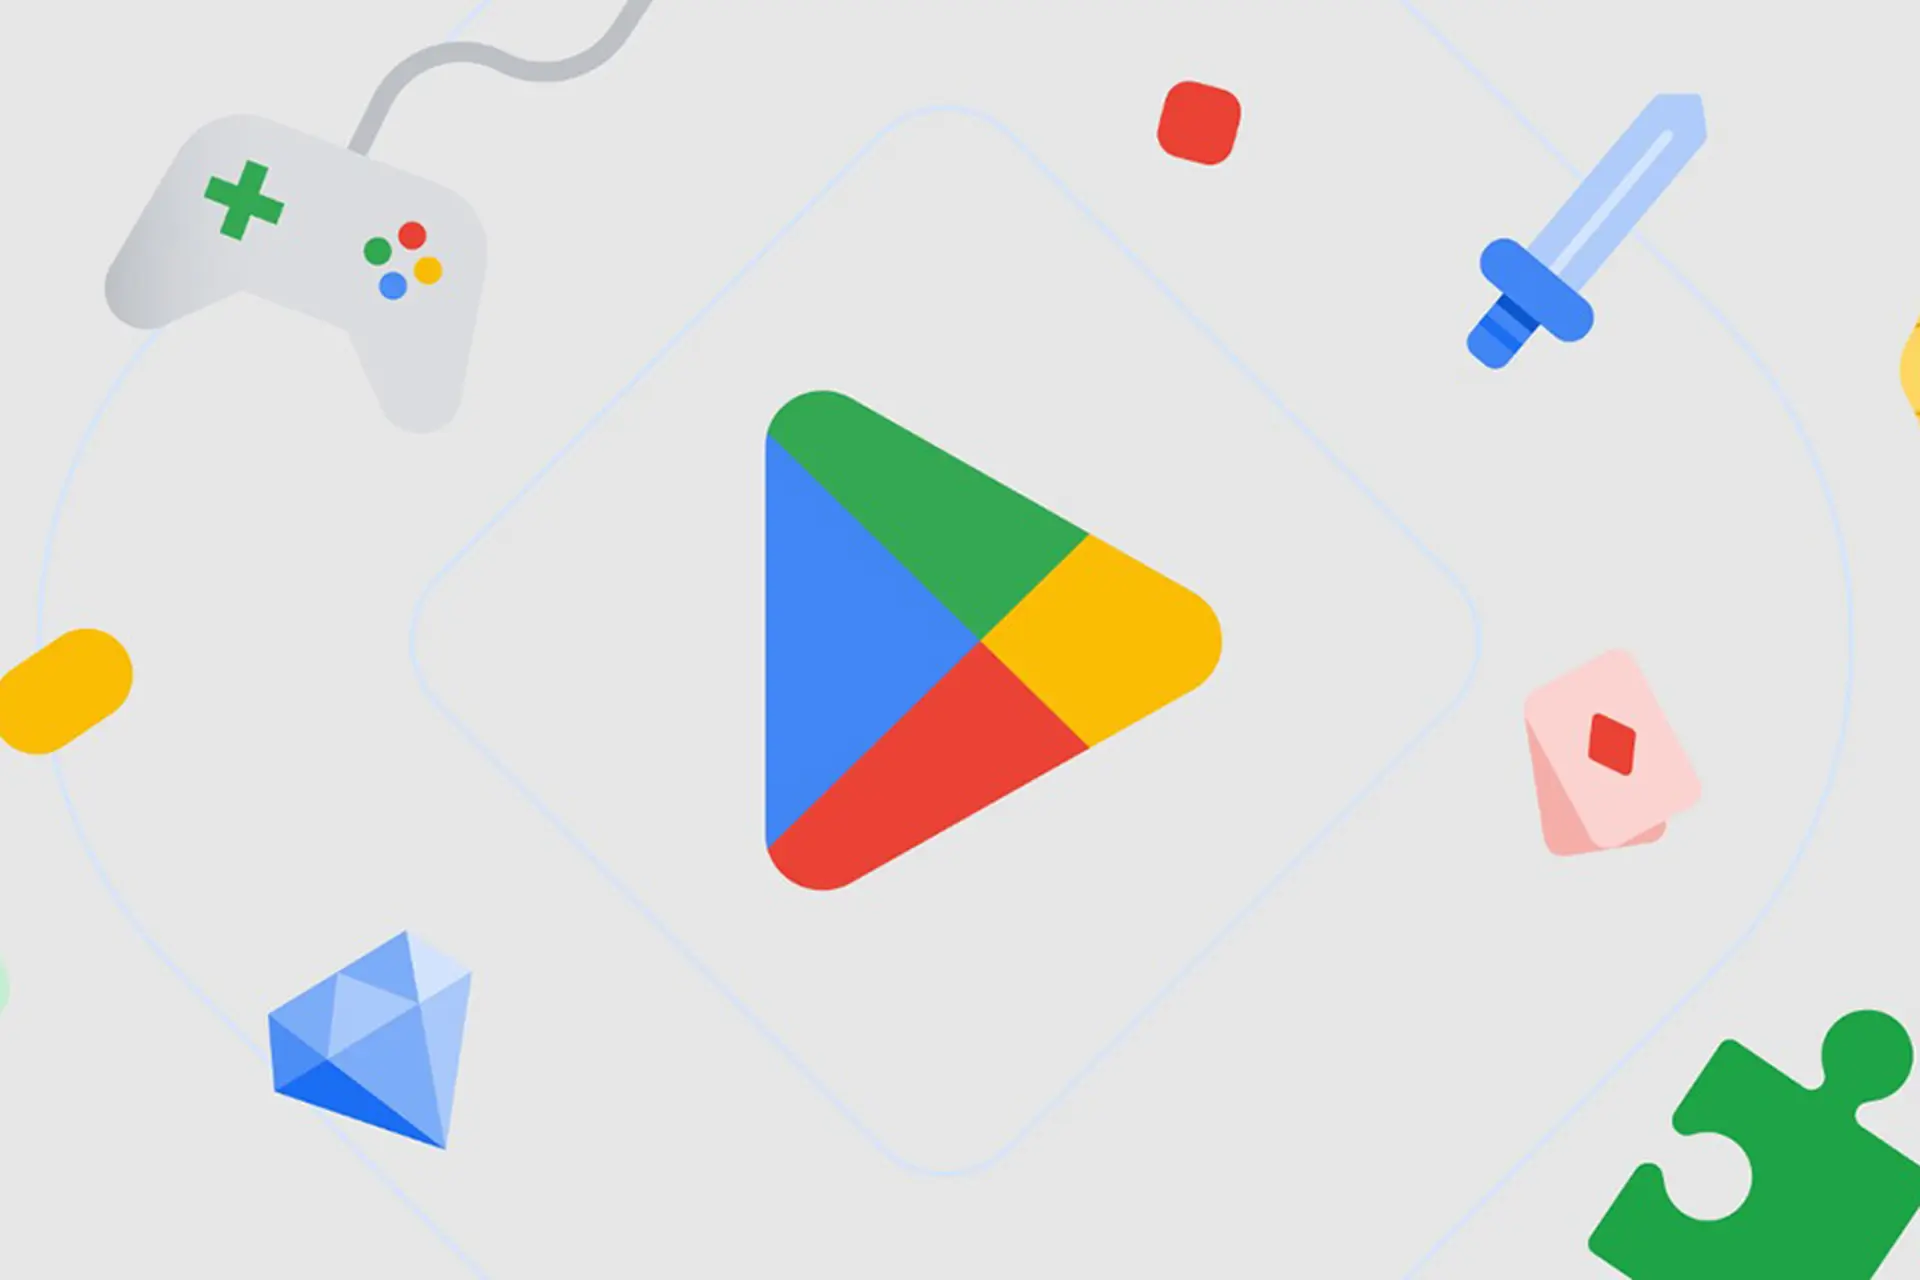
\includegraphics[width=0.95\linewidth]{figures/Phân loại-01.png}
\end{column}
\end{columns}
\end{frame}

% ------------------------------------------------------------
\subsection{Thị trường}
% ------------------------------------------------------------
\begin{frame}{Thị trường: Tổng quan}
\small
\begin{itemize}\setlength{\itemsep}{1pt}
\item Cả nước có đến \textbf{85,6 triệu} người dùng Internet (84,2\% dân số), cuối 2025
\item Trong năm 2025, Việt Nam ghi nhận \textbf{2,88 tỷ} lượt tải ứng dụng (top 11 thế giới)
\end{itemize}
\begin{center}
\scalebox{0.87}{\statcard{85,6tr}{Người dùng Internet}{84,2\% dân số, cuối 2025}\hspace{4pt}%
\statcard{2,88tỷ}{Lượt tải ứng dụng}{2025 --- top 11 thế giới}\hspace{4pt}%
\statcard{59,8\%}{Android}{thị phần HĐH di động, 9/2026}}
\end{center}
\begin{center}
\begin{tikzpicture}
% Tiêu đề tách khỏi thanh một khoảng nhìn rõ
\node[anchor=west, font=\scriptsize\bfseries, text=BKDark] at (0,0.95) {Thị phần HĐH di động (9/2026)};
% Một thanh liền: Android chiếm trước, iOS nối sau (tỉ lệ thật 59,77 : 40,19)
\fill[BKTemplate, rounded corners=3pt] (0,0.05) rectangle (7.17,0.60);
\node[font=\scriptsize\bfseries, text=white] at (3.58,0.32) {Android};
\node[font=\scriptsize, text=BKTemplate] at (3.58,-0.35) {\textbf{59,77\%}};
\fill[BKDark, rounded corners=3pt] (7.37,0.05) rectangle (12.0,0.60);
\node[font=\scriptsize\bfseries, text=white] at (9.68,0.32) {iOS};
\node[font=\scriptsize, text=BKDark] at (9.68,-0.35) {\textbf{40,19\%}};
\draw[TextGray, thick, dashed] (7.27,0.05) -- (7.27,0.60);
\end{tikzpicture}
\end{center}
\vspace{1pt}
\begin{exampleblock}{Quyết định}
Lựa chọn triển khai trên Android trước khi làm iOS hay đa nền tảng.
\end{exampleblock}
\end{frame}

% ------------------------------------------------------------
\begin{frame}{Thị trường: Từng phân hệ}
\footnotesize
\begin{columns}[T]
% ================= LEFT: VIDEO =================
\begin{column}{0.48\textwidth}
\begin{block}{Video}
{\scriptsize\color{TextGray} Xem phim (Decision Lab Q2/2024)}\\[1pt]
\begin{tikzpicture}[bar/.style={rounded corners=1pt}]
  \node[anchor=east, font=\tiny] at (0,0) {YouTube};
  \fill[BKTemplate] (0.15,0) rectangle +(3.4,0.22);
  \node[anchor=west, font=\tiny\bfseries, text=BKTemplate] at (3.65,0.11) {68\%};
  \node[anchor=east, font=\tiny] at (0,-0.35) {Facebook};
  \fill[BKLight!60] (0.15,-0.46) rectangle +(1.6,0.22);
  \node[anchor=west, font=\tiny, text=TextGray] at (1.85,-0.35) {32\%};
  \node[anchor=east, font=\tiny] at (0,-0.70) {FPT Play};
  \fill[BKLight!50] (0.15,-0.81) rectangle +(1.45,0.22);
  \node[anchor=west, font=\tiny, text=TextGray] at (1.70,-0.70) {29\%};
  \node[anchor=east, font=\tiny] at (0,-1.05) {Netflix};
  \fill[BKLight!40] (0.15,-1.16) rectangle +(1.4,0.22);
  \node[anchor=west, font=\tiny, text=TextGray] at (1.65,-1.05) {28\%};
\end{tikzpicture}\\[2pt]
{\scriptsize\color{TextGray} Số người dùng: YouTube 62,1tr $\cdot$ TikTok 76,1tr (18+)}
\end{block}
\vspace{1pt}
\begin{block}{Âm nhạc}
{\scriptsize\color{TextGray} Nghe nhạc (Decision Lab Q1/2024)}\\[1pt]
\begin{tikzpicture}[bar/.style={rounded corners=1pt}]
  \node[anchor=east, font=\tiny] at (0,0) {YouTube};
  \fill[BKTemplate] (0.15,0) rectangle +(3.85,0.22);
  \node[anchor=west, font=\tiny\bfseries, text=BKTemplate] at (4.10,0.11) {77\%};
  \node[anchor=east, font=\tiny] at (0,-0.35) {Zing MP3};
  \fill[BKLight!60] (0.15,-0.46) rectangle +(2.6,0.22);
  \node[anchor=west, font=\tiny, text=TextGray] at (2.85,-0.35) {52\%};
  \node[anchor=east, font=\tiny] at (0,-0.70) {NhacCuaTui};
  \fill[BKLight!50] (0.15,-0.81) rectangle +(1.6,0.22);
  \node[anchor=west, font=\tiny, text=TextGray] at (1.85,-0.70) {32\%};
  \node[anchor=east, font=\tiny] at (0,-1.05) {Spotify};
  \fill[BKLight!40] (0.15,-1.16) rectangle +(1.4,0.22);
  \node[anchor=west, font=\tiny, text=TextGray] at (1.65,-1.05) {28\%};
\end{tikzpicture}
\end{block}
\end{column}
% ================= RIGHT: NEWS + GAME =================
\begin{column}{0.48\textwidth}
\begin{block}{Tin tức}
\begin{itemize}\setlength{\itemsep}{1pt}
\item Báo riêng: VnExpress, Tuổi Trẻ, Dân trí
\item Tổng hợp: Báo Mới~--~tin từ hơn \textbf{150} báo điện tử
\end{itemize}
\end{block}
\vspace{1pt}
\begin{block}{Minigame}
\begin{tikzpicture}
  % Hai chỉ số: số đậm ở trên, chú thích ngay bên dưới (neo tây-bắc, chảy xuống)
  \node[anchor=north west, font=\footnotesize\bfseries, text=BKTemplate] at (0,1.95) {1,29 tỷ};
  \node[anchor=north west, font=\tiny, text=TextGray, text width=2.5cm, align=left] at (0,1.60)
    {lượt tải game di động 2025 (Adjust)};
  \node[anchor=north west, font=\footnotesize\bfseries, text=BKTemplate] at (3.55,1.95) {33 phút};
  \node[anchor=north west, font=\tiny, text=TextGray, text width=2.3cm, align=left] at (3.55,1.60)
    {phiên chơi game trung bình, Q1/2026};
  % Badge tăng trưởng
  \node[draw=GreenOK, fill=GreenOK!10, rounded corners=3pt, font=\tiny\bfseries, text=GreenOK!70!black, inner sep=2.5pt, anchor=west] at (0,0.50) {+15\% Q1/2026};
  \node[anchor=west, font=\tiny, text=TextGray] at (1.80,0.50) {số phiên chơi, so cùng kỳ (Adjust)};
\end{tikzpicture}
\end{block}
\end{column}
\end{columns}
\end{frame}

% ------------------------------------------------------------
\subsection{Đối thủ}
% ------------------------------------------------------------
\begin{frame}{Đối thủ trực tiếp: Những nền tảng đã gộp nhiều nội dung}
\footnotesize
\begin{columns}[T]
\begin{column}{0.32\textwidth}
\centering

\includegraphics[height=1.6cm,width=3.0cm,keepaspectratio=true]{figures/Đối thủ-Youtube.png}\\[2pt]
\begin{block}{\scriptsize\bfseries YouTube}
\begin{itemize}\setlength{\itemsep}{2pt}
\item Hệ sinh thái video lớn nhất
\item Premium: chạy nền, ngoại tuyến
\item Playables: chơi minigame nhẹ trong app
\end{itemize}
\end{block}
\end{column}
\begin{column}{0.32\textwidth}
\centering

\includegraphics[height=1.6cm,width=3.0cm,keepaspectratio=true]{figures/Đối thủ-Tiktok.png}\\[2pt]
\begin{block}{\scriptsize\bfseries TikTok}
\begin{itemize}\setlength{\itemsep}{2pt}
\item Video ngắn số 1
\item Minigame trong app
\item TikTok Music đóng cửa 28/11/2024 (5 thị trường, không gồm Việt Nam)
\end{itemize}
\end{block}
\end{column}
\begin{column}{0.32\textwidth}
\centering

\includegraphics[height=1.6cm,width=3.0cm,keepaspectratio=true]{figures/Đối thủ-Mocha.png}\\[2pt]
\begin{block}{\scriptsize\bfseries Mocha}
\begin{itemize}\setlength{\itemsep}{2pt}
\item Siêu ứng dụng liên lạc \& giải trí
\item Data miễn phí cho thuê bao Viettel
\item Nghe nhạc, xem video, xem phim, livestream, game
\end{itemize}
\end{block}
\end{column}
\end{columns}
\end{frame}

% ------------------------------------------------------------
\begin{frame}{Đối thủ gián tiếp: Mỗi app một phân hệ}
\footnotesize
\begin{columns}[T]
\begin{column}{0.48\textwidth}
\begin{block}{Âm nhạc}
Spotify, Zing MP3, NhacCuaTui --- mỗi app giữ một mảnh ghép
\end{block}
\vspace{1pt}
\begin{block}{Video}
Netflix, FPT Play --- nền tảng video chuyên biệt
\end{block}
\end{column}
\begin{column}{0.48\textwidth}
\begin{block}{Tin tức}
VnExpress, Tuổi Trẻ, Báo Mới --- mỗi app một nguồn tin
\end{block}
\vspace{1pt}
\begin{block}{Minigame}
Shopee (quiz, ticket game) --- gamification trong app thương mại
\end{block}
\end{column}
\end{columns}
\end{frame}

% ------------------------------------------------------------
\begin{frame}{Đối thủ: Ma trận tính năng}
\small
\centering
\begin{tabular}{@{}p{2.3cm}cccc@{}}
\toprule
\textbf{Ứng dụng} & \textbf{Video} & \textbf{Nhạc} & \textbf{Tin tức} & \textbf{Minigame} \\
\midrule
YouTube & \cmark & \pmark$^{\text{\tiny Premium}}$ & \xmark & \pmark$^{\text{\tiny Playables}}$ \\
TikTok & \cmark & \pmark$^{\text{\tiny qua sound}}$ & \xmark & \pmark \\
Mocha & \cmark & \cmark$^{\text{\tiny Keeng}}$ & \cmark & \cmark \\
Spotify/Zing & \xmark & \cmark & \pmark$^{\text{\tiny podcast}}$ & \xmark \\
Báo Mới & \xmark & \xmark & \cmark & \xmark \\
Shopee & \xmark & \xmark & \xmark & \pmark$^{\text{\tiny quiz}}$ \\
\midrule
\rowcolor{LightBG}
\textbf{Đề xuất} & \textbf{\cmark} & \textbf{\cmark} & \textbf{\cmark} & \textbf{\cmark} \\
\bottomrule
\end{tabular}

\vspace{0.12cm}
{\scriptsize \cmark~có \quad \pmark~một phần / kèm điều kiện \quad \xmark~không có}

\vspace{0.12cm}
\begin{block}{Khoảng trống}
\footnotesize Mocha hướng tới đủ bốn loại nội dung nhưng \textbf{không liên kết} chúng với nhau; các ứng dụng còn lại mỗi app một phân hệ. Không ai cho nội dung \textbf{phối hợp với nhau}.
\end{block}
\end{frame}

% ------------------------------------------------------------
\subsection{SWOT}
% ------------------------------------------------------------
\begin{frame}{SWOT}
\begin{center}
\begin{tikzpicture}[
    qbodys/.style={rounded corners=4pt, draw=GreenOK!70, fill=GreenOK!6, thick},
    qbodyw/.style={rounded corners=4pt, draw=OrangeWarn!70, fill=OrangeWarn!6, thick},
    qbodyo/.style={rounded corners=4pt, draw=BKLight!70, fill=BKLight!6, thick},
    qbodyt/.style={rounded corners=4pt, draw=RedNo!70, fill=RedNo!6, thick},
    qhead/.style={rounded corners=3pt}]
  \begin{scope}[shift={(0,3.15)}]
    \draw[qbodys] (0,0) rectangle (6.7,2.95);
    \fill[GreenOK,qhead] (0.07,2.42) rectangle (6.63,2.88);
    \node[anchor=west, font=\scriptsize\bfseries, text=white] at (0.3,2.65) {S~--~Điểm mạnh};
    \node[anchor=north west, text width=6.1cm, align=left, font=\tiny] at (0.3,2.28) {%
      \begin{itemize}\itemsep2pt
        \item[S1] Một tài khoản cho bốn phân hệ; nhạc không ngắt khi chuyển tab
        \item[S2] Playlist trộn nhạc, video, tin; chuyển nội dung sang dạng nghe
        \item[S3] Minigame từ nội dung: đố tin, đoán bài hát, karaoke
        \item[S4] Gamification chung: nhiệm vụ, streak, thú ảo
      \end{itemize}};
  \end{scope}
  \begin{scope}[shift={(6.9,3.15)}]
    \draw[qbodyw] (0,0) rectangle (6.7,2.95);
    \fill[OrangeWarn,qhead] (0.07,2.42) rectangle (6.63,2.88);
    \node[anchor=west, font=\scriptsize\bfseries, text=white] at (0.3,2.65) {W~--~Điểm yếu};
    \node[anchor=north west, text width=6.1cm, align=left, font=\tiny] at (0.3,2.28) {%
      \begin{itemize}\itemsep2pt
        \item[W1] Kho nội dung nhỏ; không ngân sách mua bản quyền
        \item[W2] Phân hệ nông hơn ứng dụng chuyên biệt, nhất là gợi ý
        \item[W3] Gộp bốn phân hệ tăng dung lượng, chậm khởi động
        \item[W4] Thương hiệu mới, nhóm nhỏ, thời gian có hạn
      \end{itemize}};
  \end{scope}
  \begin{scope}[shift={(0,0)}]
    \draw[qbodyo] (0,0) rectangle (6.7,2.95);
    \fill[BKLight,qhead] (0.07,2.42) rectangle (6.63,2.88);
    \node[anchor=west, font=\scriptsize\bfseries, text=white] at (0.3,2.65) {O~--~Cơ hội};
    \node[anchor=north west, text width=6.1cm, align=left, font=\tiny] at (0.3,2.28) {%
      \begin{itemize}\itemsep2pt
        \item[O1] 85,6 triệu người dùng Internet, mạng tốc độ cao
        \item[O2] Retention giải trí chỉ 1\% sau 30 ngày~--~vấn đề chung
        \item[O3] Gamification quen thuộc qua MoMo, Shopee
        \item[O4] YouTube nền cần Premium; TikTok Music đã đóng
      \end{itemize}};
  \end{scope}
  \begin{scope}[shift={(6.9,0)}]
    \draw[qbodyt] (0,0) rectangle (6.7,2.95);
    \fill[RedNo,qhead] (0.07,2.42) rectangle (6.63,2.88);
    \node[anchor=west, font=\scriptsize\bfseries, text=white] at (0.3,2.65) {T~--~Thách thức};
    \node[anchor=north west, text width=6.1cm, align=left, font=\tiny] at (0.3,2.28) {%
      \begin{itemize}\itemsep1pt
        \item[T1] Đối thủ lớn đã có minigame, sao chép nhanh
        \item[T2] Bản quyền nhạc, video; tổng hợp tin cần giấy phép
        \item[T3] Điểm thưởng không được quy đổi ra tiền
        \item[T4] Luật BVDLCN 2025 chặt hơn về đồng ý
        \item[T5] Người dùng ngại rời playlist, lịch sử cũ
      \end{itemize}};
  \end{scope}
\end{tikzpicture}
\end{center}
\end{frame}

% ------------------------------------------------------------
\subsection{User Personas}
% ------------------------------------------------------------
\begin{frame}{User Personas (1/3)}
\linespread{0.88}%
\begin{columns}[T]
\begin{column}{0.48\textwidth}
\begin{block}{\small Minh Anh~--~21, sinh viên \tiny(Primary)}
{\tiny\color{TextGray} 21, sinh viên đại học $\cdot$ TP.\ HCM $\cdot$ công nghệ cao $\cdot$ Android 6~GB $\cdot$ 3--5 giờ/ngày}\par\vspace{0.6mm}
{\tiny\textbf{Mục tiêu:} dùng nhiều loại nội dung trong một app; xem video khi đọc tin; nghe nhạc khi lướt tin hoặc chơi game; chuyển đổi nhanh; giảm số lần mở/đóng app}\par\vspace{0.4mm}
{\tiny\textbf{Pain:} liên tục chuyển app; nội dung bị dừng khi đổi hoạt động; khó tìm lại video/bài đang xem; PIP che nội dung; âm thanh chồng nhau}\par\vspace{0.4mm}
{\tiny\textbf{Hành vi:} giải trí giờ nghỉ và buổi tối; quen vuốt, chạm, kéo thả; thích nội dung tiếp tục từ chỗ cũ; thường làm một việc chính + một việc phụ}\par\vspace{0.4mm}
{\tiny\textbf{Tình huống:} Đang xem video, muốn đọc bài báo mới. Chạm tab Tin $\rightarrow$ video tự thu PIP, kéo sang góc khác khỏi đoạn văn. Đọc xong, chạm PIP quay lại video phát tiếp đúng vị trí.}
\end{block}
\end{column}
\begin{column}{0.48\textwidth}
\begin{block}{\small Hoàng Nam~--~27, nhân viên văn phòng}
{\tiny\color{TextGray} 27, nhân viên văn phòng $\cdot$ TP.\ HCM $\cdot$ công nghệ TB--khá $\cdot$ Android 8~GB $\cdot$ 1--2 giờ/ngày}\par\vspace{0.6mm}
{\tiny\textbf{Mục tiêu:} đọc nhanh tin trong giờ nghỉ; nghe nhạc khi di chuyển; tiếp tục bài viết trước đó bằng ít thao tác; điều khiển âm thanh từ notification hoặc màn hình khoá}\par\vspace{0.4mm}
{\tiny\textbf{Pain:} không có thời gian tìm nội dung; thao tác nhiều màn gây bất tiện; âm thanh gián đoạn khi có cuộc gọi; phải tìm lại bài đang nghe/đọc; giao diện nhiều tùy chọn gây rối}\par\vspace{0.4mm}
{\tiny\textbf{Hành vi:} dùng khi di chuyển, nghỉ trưa, sau giờ làm; nghe nhạc qua tai nghe Bluetooth; thói quen khoá màn khi nghe; thích nút điều khiển rõ ràng}\par\vspace{0.4mm}
{\tiny\textbf{Tình huống:} Trên đường đến công ty, phát playlist rồi khoá điện thoại. Nghỉ trưa mở app đọc tin, nhạc vẫn phát, điều khiển qua dock. Có cuộc gọi, app tự nhường; sau cuộc gọi nhạc phát lại đúng chỗ.}
\end{block}
\end{column}
\end{columns}
\end{frame}

% ------------------------------------------------------------
\begin{frame}{User Personas (2/3)}
\linespread{0.88}%
\begin{columns}[T]
\begin{column}{0.48\textwidth}
\begin{block}{\small Quốc Huy~--~19, sinh viên năm nhất}
{\tiny\color{TextGray} 19, sinh viên năm nhất $\cdot$ Bình Dương $\cdot$ công nghệ trung bình $\cdot$ Android 3~GB $\cdot$ dữ liệu giới hạn}\par\vspace{0.6mm}
{\tiny\textbf{Mục tiêu:} chơi minigame đơn giản; nghe nhạc khi chơi game; chơi tiếp khi mất mạng; không mất tiến độ; hạn chế giật lag; tiết kiệm dữ liệu}\par\vspace{0.4mm}
{\tiny\textbf{Pain:} máy chậm khi nhiều tác vụ; mạng không ổn định; game mất tiến độ khi app bị đóng; video HQ tốn dữ liệu; âm game xung đột nhạc nền}\par\vspace{0.4mm}
{\tiny\textbf{Hành vi:} chơi game giờ nghỉ; ưu tiên game nhẹ, ngắn; mở nhạc khi chơi; chọn chất lượng thấp để tiết kiệm data}\par\vspace{0.4mm}
{\tiny\textbf{Tình huống:} Đang nghe nhạc, vào Games mở 2048. Nhạc vẫn phát, âm game tự nhỏ nhường nhạc. Mạng ngắt nhưng game vẫn chạy offline. Chuyển sang Tin đọc bài đã lưu, app tạm dừng game giữ ván dở. Quay lại, ván dở tự hiện lại.}
\end{block}
\end{column}
\begin{column}{0.48\textwidth}
\begin{block}{\small Thảo Vy~--~24, nhân viên marketing}
{\tiny\color{TextGray} 24, nhân viên marketing $\cdot$ TP.\ HCM $\cdot$ công nghệ cao $\cdot$ Android 8~GB $\cdot$ Wi-Fi + 5G}\par\vspace{0.6mm}
{\tiny\textbf{Mục tiêu:} khám phá nội dung mới; chuyển đổi giữa video và bài báo cùng chủ đề; tìm kiếm trên nhiều phân hệ; lưu nội dung xem sau; tiếp tục từ chỗ cũ}\par\vspace{0.4mm}
{\tiny\textbf{Pain:} nội dung cùng chủ đề nằm rải rác trên nhiều app; phải tìm lại chủ đề khi chuyển video sang tin; khó quản lý danh sách xem sau; dễ mất dấu nội dung đã xem}\par\vspace{0.4mm}
{\tiny\textbf{Hành vi:} xem video, đọc báo, tìm chủ đề mới; hay dùng search và bộ lọc; chuyển từ nội dung này sang nội dung liên quan}\par\vspace{0.4mm}
{\tiny\textbf{Tình huống:} Đang đọc bài báo về công nghệ mới. Muốn xem video liên quan, dùng Search xuyên nội dung. Vị trí đọc được lưu. Xem video xong quay lại Tin, app khôi phục đúng đoạn cũ. Đánh dấu cả bài và video xem cuối tuần.}
\end{block}
\end{column}
\end{columns}
\end{frame}

% ------------------------------------------------------------
\begin{frame}{User Personas (3/3)}
\linespread{0.88}%
\begin{columns}[T]
\begin{column}{0.48\textwidth}
\begin{block}{\small Gia Bảo~--~23, sinh viên CNTT}
{\tiny\color{TextGray} 23, sinh viên CNTT $\cdot$ TP.\ HCM $\cdot$ công nghệ rất cao $\cdot$ Android 12~GB $\cdot$ Wi-Fi + 5G}\par\vspace{0.6mm}
{\tiny\textbf{Mục tiêu:} chủ động chọn cách chuyển tab; điều khiển trạng thái phát; tùy chỉnh vị trí PIP; quyết định giữ video khi vào game; quản lý âm thanh theo từng hoạt động}\par\vspace{0.4mm}
{\tiny\textbf{Pain:} app tự dừng/tiếp tục không đúng ý; không có tùy chọn đổi hành vi chuyển màn; PIP kích thước cố định; khó biết nguồn âm nào đang phát; phải thao tác nhiều để đổi cài đặt}\par\vspace{0.4mm}
{\tiny\textbf{Hành vi:} quen cài đặt nâng cao; trải nghiệm nhiều app đa phương tiện; chấp nhận giao diện phức tạp nếu tổ chức rõ}\par\vspace{0.4mm}
{\tiny\textbf{Tình huống:} Xem video và muốn chơi minigame, đã thiết lập ``giữ PIP khi vào Games''. Mở game, video tự thu nhỏ. Sau đó phát nhạc: app dừng video, ưu tiên bài mới. Quay lại video qua trình điều khiển.}
\end{block}
\end{column}
\begin{column}{0.48\textwidth}
\begin{block}{\small Thu Hà~--~37, nhân viên hành chính}
{\tiny\color{TextGray} 37, nhân viên hành chính $\cdot$ Đồng Nai $\cdot$ công nghệ trung bình $\cdot$ Android 4~GB $\cdot$ Wi-Fi + 4G}\par\vspace{0.6mm}
{\tiny\textbf{Mục tiêu:} đọc tin trên giao diện rõ ràng; điều khiển nhạc bằng nút quen thuộc; biết nội dung nào đang hoạt động; dừng hoặc đóng trình phát bất cứ lúc nào; tăng cỡ chữ khi đọc}\par\vspace{0.4mm}
{\tiny\textbf{Pain:} biểu tượng không nhãn; chữ nhỏ hoặc tương phản thấp; không biết âm phát từ đâu; PIP che nội dung; lo nhấn nhầm mất bài đang đọc}\par\vspace{0.4mm}
{\tiny\textbf{Hành vi:} dùng trong nhà và lúc nghỉ; đọc tin, xem video, nghe nhạc nhiều hơn chơi game; ưu tiên nút bấm rõ hơn cử chỉ; thường dùng một tay}\par\vspace{0.4mm}
{\tiny\textbf{Tình huống:} Mở app đọc bài báo, tăng cỡ chữ bằng nút A+. Mở video liên quan hiện PIP. Muốn tập trung đọc, nhấn ``Tạm dừng video'', app hiển thị video đã dừng, tiếp tục đọc đúng chỗ cũ.}
\end{block}
\end{column}
\end{columns}
\end{frame}

% ------------------------------------------------------------
\subsection{USP \& Winning Zone}
% ------------------------------------------------------------
\begin{frame}{USP \& Winning Zone}
\begin{center}
\begin{tikzpicture}[scale=0.70]
  \begin{scope}
    \clip (0,2.2) circle (2.6);
    \clip (-1.905,-1.1) circle (2.6);
    \fill[AccentGold, opacity=0.35] (-4,-2) rectangle (4,5);
  \end{scope}
  \fill[RedNo, opacity=0.18] (1.905,-1.1) circle (2.6);
  \fill[BKLight, opacity=0.10] (0,2.2) circle (2.6);
  \fill[GreenOK, opacity=0.10] (-1.905,-1.1) circle (2.6);
  \draw[BKLight, very thick] (0,2.2) circle (2.6);
  \draw[GreenOK, very thick] (-1.905,-1.1) circle (2.6);
  \draw[RedNo, very thick] (1.905,-1.1) circle (2.6);
  \node[align=center, font=\small\bfseries, text=BKLight] at (0,3.45) {Nhu cầu\\người dùng};
  \node[align=center, font=\small\bfseries, text=GreenOK!60!black] at (-3.2,-1.6) {Thế mạnh\\đề xuất};
  \node[align=center, font=\small\bfseries, text=RedNo] at (3.2,-1.6) {Thế mạnh\\đối thủ};
  \node[fill=AccentGold!25, draw=black!40, rounded corners=2pt, inner sep=4pt] at (-1.4,0.7) {\small\textbf{Winning Zone}};
\end{tikzpicture}
\end{center}
\vfill
\begin{center}\small
Nhu cầu $\cap$ thế mạnh của đề xuất, \textbf{nằm ngoài} vùng đối thủ đã phủ
\end{center}
\end{frame}

% ------------------------------------------------------------
\begin{frame}{USP \& Winning Zone}
\begin{center}
\begin{tikzpicture}[
    needc/.style={rounded corners=4pt, draw=BKLight!70, fill=BKLight!6, thick},
    ourc/.style={rounded corners=4pt, draw=GreenOK!70, fill=GreenOK!6, thick},
    compc/.style={rounded corners=4pt, draw=RedNo!70, fill=RedNo!6, thick},
    hstrip/.style={rounded corners=3pt}]
  % ---- Nhu cầu người dùng ----
  \begin{scope}[shift={(0,0)}]
    \draw[needc] (0,0) rectangle (4.4,3.4);
    \fill[BKLight,hstrip] (0.07,2.92) rectangle (4.33,3.33);
    \node[anchor=west, font=\scriptsize\bfseries, text=white] at (0.25,3.12) {Nhu cầu người dùng};
    \node[anchor=north west, text width=3.9cm, align=left, font=\tiny] at (0.25,2.78) {%
      \begin{itemize}\itemsep1pt
        \item Chỉ cài và đăng \textbf{một} ứng dụng duy nhất
        \item Chuyển đổi loại nội dung \textbf{không gián đoạn}
        \item Dùng được \textbf{hai loại nội dung song song}
        \item Tiết kiệm dung lượng, RAM và pin
      \end{itemize}};
  \end{scope}
  % ---- Thế mạnh của đề xuất ----
  \begin{scope}[shift={(4.6,0)}]
    \draw[ourc] (0,0) rectangle (4.4,3.4);
    \fill[GreenOK,hstrip] (0.07,2.92) rectangle (4.33,3.33);
    \node[anchor=west, font=\scriptsize\bfseries, text=white] at (0.25,3.12) {Thế mạnh của đề xuất};
    \node[anchor=north west, text width=3.9cm, align=left, font=\tiny] at (0.25,2.78) {%
      \begin{itemize}\itemsep1pt
        \item Bốn phân hệ dùng chung \textbf{một media engine}
        \item \textbf{Dock mini player} xuyên suốt
        \item Song song hai nội dung, popup xác nhận khi xung đột âm thanh
        \item Chuyển đổi hình thức: video $\rightarrow$ mp3, báo $\rightarrow$ audio
        \item Minigame sinh từ nội dung đang xem, điểm thưởng dùng chung
      \end{itemize}};
  \end{scope}
  % ---- Thế mạnh đối thủ ----
  \begin{scope}[shift={(9.2,0)}]
    \draw[compc] (0,0) rectangle (4.4,3.4);
    \fill[RedNo,hstrip] (0.07,2.92) rectangle (4.33,3.33);
    \node[anchor=west, font=\scriptsize\bfseries, text=white] at (0.25,3.12) {Thế mạnh đối thủ};
    \node[anchor=north west, text width=3.9cm, align=left, font=\tiny] at (0.25,2.78) {%
      \begin{itemize}\itemsep1pt
        \item Kho bản quyền lớn (phim HD, Keeng)
        \item Cơ sở người dùng khổng lồ (Mocha 16 triệu)
        \item Data miễn phí thuê bao nhà mạng
        \item Mạng xã hội chat + voice sticker
        \item {\color{TextGray}\itshape Vùng không cạnh tranh trực diện}
      \end{itemize}};
  \end{scope}
\end{tikzpicture}
\end{center}
\vfill
\end{frame}

% ------------------------------------------------------------
\begin{frame}{USP \& Winning Zone}
\small
\centering
\begin{tabular}{@{}p{0.5cm}p{3.4cm}p{8.4cm}@{}}
\toprule
 & \textbf{Nội dung} & \textbf{Biểu hiện cụ thể} \\
\midrule
W1 & Xuyên phân hệ & Dock mini dùng chung 4 loại nội dung; một tài khoản; trạng thái giữ nguyên khi đổi tab \\
W2 & Song song hoá & Nghe nhạc khi đọc tin; PIP video khi lướt; popup xác nhận khi xung đột âm thanh \\
W3 & Converting & Nhấn giữ video $\rightarrow$ trích mp3; bài báo $\rightarrow$ audio ``nghe tin'' \\
W4 & Game gắn nội dung & Đoán bài hát từ kho nhạc; quiz từ bài báo đang đọc \\
W5 & Gamification & Nhiệm vụ, streak, thú cưng, điểm thưởng dùng chung bốn phân hệ \\
W6 & Tổng kết cá nhân & Thẻ tổng kết hoạt động trong tháng, xuất ảnh chia sẻ \\
\bottomrule
\end{tabular}
\end{frame}

% ------------------------------------------------------------
\begin{frame}{Unique Selling Point}
\vspace{2mm}
\begin{exampleblock}{Phát biểu Unique Selling Point}
\small\itshape
Ứng dụng giải trí ``4 trong 1'' trên Android: \textbf{chuyển đổi, chạy song song và chuyển đổi hình thức} giữa video, nhạc, tin tức và minigame trong cùng một app. Ngoài ra có \textbf{hệ thống gamification}: nhiệm vụ mỗi ngày, streak, thú cưng ảo và điểm thưởng dùng chung cho cả bốn phân hệ.
\end{exampleblock}
\vspace{4mm}
\end{frame}
